\documentclass[12pt]{report}
\usepackage[utf8]{inputenc}
\usepackage[russian]{babel}
%\usepackage[14pt]{extsizes}
\usepackage{listings}
\usepackage{graphicx}
\usepackage{amsmath,amsfonts,amssymb,amsthm,mathtools} 
\usepackage{pgfplots}
\usepackage{filecontents}
\usepackage{indentfirst}
\usepackage{eucal}
\usepackage{amsmath}
\usepackage{enumitem}
\usepackage{fixltx2e}
\usepackage{float}

\frenchspacing

\usepackage{indentfirst} % Красная строка


%\usetikzlibrary{datavisualization}
%\usetikzlibrary{datavisualization.formats.functions}

\usepackage{amsmath}


% Для листинга кода:
\lstset{ %
language=caml,                 % выбор языка для подсветки (здесь это С)
basicstyle=\small\sffamily, % размер и начертание шрифта для подсветки кода
numbers=left,               % где поставить нумерацию строк (слева\справа)
numberstyle=\tiny,           % размер шрифта для номеров строк
stepnumber=1,                   % размер шага между двумя номерами строк
numbersep=5pt,                % как далеко отстоят номера строк от подсвечиваемого кода
showspaces=false,            % показывать или нет пробелы специальными отступами
showstringspaces=false,      % показывать или нет пробелы в строках
showtabs=false,             % показывать или нет табуляцию в строках
frame=single,              % рисовать рамку вокруг кода
tabsize=2,                 % размер табуляции по умолчанию равен 2 пробелам
captionpos=t,              % позиция заголовка вверху [t] или внизу [b] 
breaklines=true,           % автоматически переносить строки (да\нет)
breakatwhitespace=false, % переносить строки только если есть пробел
escapeinside={\#*}{*)}   % если нужно добавить комментарии в коде
}

\usepackage[left=2cm,right=2cm, top=2cm,bottom=2cm,bindingoffset=0cm]{geometry}


% plot
\usepackage{pgfplots}
\usepackage{filecontents}
\usetikzlibrary{datavisualization}
\usetikzlibrary{datavisualization.formats.functions}

\graphicspath{ {img/} }


\usepackage{subcaption}

\captionsetup{labelsep=endash}
\captionsetup[figure]{name={Рисунок}}


\begin{document}
	\begin{titlepage}
		\thispagestyle{empty}
		
		\noindent
		\begin{minipage}{0.15\textwidth}
			
\includegraphics[width=\linewidth]{main_logo}
		\end{minipage}
		\noindent
		\begin{minipage}{0.9\textwidth}
			\centering
			\textbf{Министерство науки и высшего образования Российской Федерации}\\
			\textbf{Федеральное государственное бюджетное образовательное учреждение высшего образования}\\
			\textbf{«Московский государственный технический университет имени Н.Э.~Баумана}\\
			\textbf{(национальный исследовательский университет)»}\\
			\textbf{(МГТУ им. Н.Э.~Баумана)}
		\end{minipage}
		
		\noindent
		\rule{18cm}{3pt} %пустая строка
		\newline\newline %пустая строка
		\noindent ФАКУЛЬТЕТ $\underline{\text{«Информатика и системы управления»}}$ \newline\newline
		\noindent КАФЕДРА $\underline{\text{«Программное обеспечение ЭВМ и информационные технологии»}}$\newline\newline\newline\newline\newline
		
		
		\begin{center}
			\noindent\begin{minipage}{1.3\textwidth}\centering
				\Large\textbf{  Отчёт о лабораторной работе №2}\newline
				\textbf{по дисциплине "Анализ алгоритмов"}\newline
				\textbf{на тему "Умножение матриц"}\newline\newline
			\end{minipage}
		\end{center}
		
		\noindent\textbf{Студент} $\underline{\text{Коняев Е.А}}$\newline\newline
		\noindent\textbf{Группа} $\underline{\text{ИУ7-53Б}}$\newline\newline
		\noindent\textbf{Преподаватели} $\underline{\text{Волкова Л.Л., Строганов Ю.В.}}$\newline\newline
		\noindent\textbf{Дата сдачи отчета}$\underline{\text{~~~~~~~~~~~~~~~~~~~~~~~~~~~}}$\newline\newline
		\noindent\textbf{Оценка (баллы)} $\underline{\text{~~~~~~~~~~~~~~~~~~~~~~~~~~~}}$\newline\newline\newline
		
		\begin{center}
			\vfill
			Москва~---~\the\year~г.
		\end{center}
	\end{titlepage}
	
	\setcounter{page}{2}
	\tableofcontents
	
	\newpage
	\chapter*{Введение}
	
	\addcontentsline{toc}{chapter}{Введение}

Матрица -- это математический объект, который представляет собой таблицу чисел из определенного количества строк и столбцов.

Операции обработки матриц, а в частности их умножение, является одной из самых фундаментальных операций в современных вычислениях. Оно выполняется миллиарды раз в день по всему миру в вычислениях для линейной алгебры, статистики, биоинформатики, физики и разных других областей науки, техники и обработки сигналов и образов.

Умножение двух матриц возможно только в том случае, если число столбцов первой матрицы совпадает с числом строк во второй. Результирующая матрица будет иметь столько же строк, сколько в первой матрице, и столько же столбцов, сколько во второй. При этом данная операция не является в общем случае коммутативной.

	
	\chapter{Аналитическая часть}
	
	\section{Цель и задачи}
	
	Целью данной работой является изучение и реализация алгоритмов умножения матриц, вычисление трудоемкости этих алгоритмов. В данной лабораторной работе рассматривается стандартный алгоритм умножения матриц, алгоритм Винограда и модифицированный алгоритм Винограда. Для достижения поставленной цели требуется решить следующие задачи:
	
	\begin{enumerate}
		\item[1)] изучить и рассмотреть алгоритм классического умножения матриц, алгоритм Винограда и модифицированный алгоритм Винограда; 
		\item[2)] построить блок-схемы данных алгоритмов;
		\item[3)] реализовать каждый из алгоритмов;
		\item[4)] оценить трудоемкость алгоритмов;
		\item[5)] экспериментально оценить временные характеристики алгоритмов;
		\item[6)] сделать вывод на основании проделанной работы.
	\end{enumerate}
	
	
	\section{Стандартный алгоритм}
	
	Пусть даны две прямоугольные матрицы
	\begin{equation}
		A_{lm} = \begin{pmatrix}
			a_{11} & a_{12} & \ldots & a_{1m}\\
			a_{21} & a_{22} & \ldots & a_{2m}\\
			\vdots & \vdots & \ddots & \vdots\\
			a_{l1} & a_{l2} & \ldots & a_{lm}
		\end{pmatrix},
		\quad
			B_{mn} = \begin{pmatrix}
			b_{11} & b_{12} & \ldots & b_{1n}\\
			b_{21} & b_{22} & \ldots & b_{2n}\\
			\vdots & \vdots & \ddots & \vdots\\
			b_{m1} & b_{m2} & \ldots & b_{mn}
		\end{pmatrix},
	\end{equation}\newline\newline\newline\newline\newline\newline\newline

	тогда матрица $C$, полученная в результате умножения этих матриц, будет иметь вид
	
	\begin{equation}
		C_{ln} = \begin{pmatrix}
			c_{11} & c_{12} & \ldots & c_{1n}\\
			c_{21} & c_{22} & \ldots & c_{2n}\\
			\vdots & \vdots & \ddots & \vdots\\
			c_{l1} & c_{l2} & \ldots & c_{ln}
		\end{pmatrix},
	\end{equation}

	где
	\begin{equation}
		\label{eq:M}
		c_{ij} =
			\sum_{r=1}^{m} a_{ir}b_{rj} \quad (i=\overline{1,l}; j=\overline{1,n})
	\end{equation}

	Стандартный алгоритм реализует данную формулу.
	
	
	\section{Алгоритм Копперсмита -- Винограда}
	
	В стандартном умножении двух матриц каждый элеменит результирующей матрицы представляет собой скалярное произведение двух векторов исходных матриц (строки из первой матрицы и столбца из второй). Такое умножение допускает предварительную обработку, которая позволяет часть вычислений выполнить заранее.
	
	Рассмотрим два вектора $V = (v_1, v_2, v_3, v_4)$ и $W = (w_1, w_2, w_3, w_4)$.
Их скалярное произведение: $V \cdot W = v_1w_1 + v_2w_2 + v_3w_3 + v_4w_4$, что эквивалентно (\ref{equal1})
\begin{equation}
	\label{equal1}
		V \cdot W = (v_1 + w_2)(v_2 + w_1) + (v_3 + w_4)(v_4 + w_3) - v_1v_2 - v_3v_4 - w_1w_2 - w_3w_4.
\end{equation}

	Хоть выражение в правой части (\ref{equal1}) имеет большее количество операций, чем стандартный алгоритм, но оно допускает предварительную обработку: его части можно вычислить заранее и запомнить для каждой строки и столбца первой и второй матрицы соответсвенно. Таким образом в рассматриваемом выше примере в процессе самого умножения требуется выполнить лишь 2 операции умножения, и 5 операций сложения (вместо 4 операций умножения и 3 операций сложения в стандартном алгоритме). Так как операция сложения выполняется в вычислительных машинах быстрее, чем умножению, то данный алгоритм по теоретической оценке должен работать быстрее, чем стандартный алгоритм умножения матриц. 
	
	\section*{Вывод}
	
	В данном разделе были рассмотрены алгоритмы классического умножения матриц и алгоритм Винограда.
	
	\chapter{Конструкторская часть}
	
	\section{Модель вычислений}

	Для вычисления трудоемкости будем использовать следующую модель вычислений.

	\begin{enumerate}
		\item[1)] операции из списка (\ref{for:opers1}) имеют трудоемкость 1.
		\begin{equation}
		\label{for:opers1}
		+, -, \%, ==, !=, <, >, <=, >=, [], ++, {-}-, {<}<, {>}>.
		\end{equation}
		\item[2)] операции из списка (\ref{for:opers2}) имеют трудоемкость 2.
		\begin{equation}
		\label{for:opers2}
		*, /.
		\end{equation}
		\item[3)] трудоемкость оператора выбора if условие then A else B рассчитывается, как (\ref{for:if}).
		\begin{equation}
		\label{for:if}
		f_{if} = f_{\text{условия}} +
		\begin{cases}
		f_A, & \text{условие выполняется,}\\
		f_B, & \text{иначе.}
		\end{cases}
		\end{equation}
		\item[4)] трудоемкость вызова функции равна 0.
		\item[5)] трудоемкость цикла рассчитывается, как (\ref{for:for}).
		\begin{equation}
		\label{for:for}
		f_{for} = f_{\text{инициализации}} + f_{\text{сравнения}} + N(f_{\text{тела}} + f_{\text{инкремента}} + f_{\text{сравнения}})
		\end{equation}
	\end{enumerate}
	
	\section{Трудоёмкость алгоритмов}
	
	\subsection{Стандартный алгоритм умножения матриц}
	
	Пусть $N$ -- количество строк в первой матрице, $M$ -- количество колонок во второй матрице, $Q$ -- количество колонок в первой матрице.
	Трудоёмкость стандартного алгоритма умножения матриц состоит из:\newline\newline\newline\newline\newline\newline
	
	\begin{enumerate}
		\item[1)] внешнего цикла по $i \in [0..N)$, трудоёмкость которого: $f = 2 + N \cdot (2 + f_{body})$;
		\item[2)] цикла по $j \in [0..M)$, трудоёмкость которого: $f = 2 + M \cdot (2 + f_{body})$;
		\item[3)] скалярного умножения двух векторов - цикл по $k \in [0..Q)$, трудоёмкость которого: $f = 2 + 10Q$.
	\end{enumerate}
	
	Трудоёмкость стандартного алгоритма равна трудоёмкости внешнего цикла, можно вычислить ее, подставив циклы тела (\ref{for:base})
	\begin{equation}
		\label{for:base}
		f_{base} = 2 + N \cdot (4 + M \cdot (4 + 10Q)) = 2 + 4N + 4NM + 10NMQ \approx 10NMQ
	\end{equation}
	
	\subsection{Алгоритм Копперсмита — Винограда}

	Трудоёмкость алгоритма Копперсмита — Винограда состоит из:

	\begin{enumerate}
		\item[1)] создания векторов размерами $N$ и $M$.
		\begin{equation}
		\label{for:init}
		f_{create} = N + M;
		\end{equation}
		
		\item[2)] заполнения вектора $N$.
		\begin{equation}
		\label{for:MH}
		f_{rows} = 3 + \frac{Q}{2} \cdot (5 + 12N);
		\end{equation}
		
		\item[3)] заполнения вектора cols.
		\begin{equation}
		\label{for:MV}
		f_{cols} = 3 + \frac{Q}{2} \cdot (5 + 12M);
		\end{equation}
		
		\item[4)] цикла заполнения матрицы для чётных размеров.
		\begin{equation}
		\label{for:cycle}
		f_{cycle} = 2 + N \cdot (4 + M \cdot (11 + \frac{25}{2} \cdot Q));
		\end{equation}
		
		\item[5)] цикла, для дополнения умножения суммой последних нечётных строки и столбца, если общий размер нечётный.
		\begin{equation}
		\label{for:last}
		f_{last} = \begin{cases}
		2, & \text{чётная,}\\
		4 + N \cdot (4 + 14M), & \text{иначе.}
		\end{cases}
		\end{equation}
	\end{enumerate}

	Итого, для худшего случая (нечётный размер матриц): 
	\begin{equation}
	\label{for:bad}
	f_{wino\_w} = N + M + 12 + 8N + 5Q + 6NQ + 6MQ + 25NM + \frac{25}{2}NMQ \approx 12.5 \cdot NMQ
	\end{equation}

	Для лучшего случая (чётный размер матриц): 
	\begin{equation}
	\label{for:good}
	f_{wino\_b} = N + M + 10 + 4N + 5Q + 6NQ + 6MQ + 11NM + \frac{25}{2}NMQ \approx 12.5 \cdot NMQ
	\end{equation}

	\subsection{Оптимизированный алгоритм Копперсмита — Винограда}

	Оптимизации алгоритма:
	\begin{enumerate}
		\item[1)] операции вида $x = x + k$ заменены на $x += k$;
		\item[2)] умножение и деление на 2 заменено побитовым сдвигом;
		\item[3)] происходит предвычисление некоторых слагаемых алгоритма.
	\end{enumerate}
	
	Трудоёмкость улучшенного алгоритма Копперсмита — Винограда состоит из:
	\begin{enumerate}
		\item[1)] создания векторов $N$ и $M$.
		\begin{equation}
		\label{for:impr_init}
		f_{init} = N + M;
		\end{equation}
		
		\item[2)] заполнения вектора $N$.
		\begin{equation}
		\label{for:impr_MH}
		f_{rows} = 2 + \frac{Q}{2} \cdot (4 + 8N);
		\end{equation}
		
		\item[3)] заполнения вектора $M$.
		\begin{equation}
		\label{for:impr_MV}
		f_{cols} = 2 + \frac{Q}{2} \cdot (4 + 8M);
		\end{equation}
		
		\item[4)] цикла заполнения матрицы для чётных размеров.
		\begin{equation}
		\label{for:impr_cycle}
		f_{cycle} = 2 + N \cdot (4 + M \cdot (8 + 9Q))
		\end{equation}
		
		\item[5)] цикла, для дополнения умножения суммой последних нечётных строки и столбца, если общий размер нечётный.
		\begin{equation}
		\label{for:impr_last}
		f_{last} = 
		\begin{cases}
		2, & \text{чётная,}\\
		4 + N \cdot (4 + 12M), & \text{иначе.}
		\end{cases}
		\end{equation}
	\end{enumerate}

	Итого, для худшего случая (нечётный общий размер матриц) имеем:
	\begin{equation}
	\label{for:bad_impr}
	f = N + M + 10 + 4Q + 4QM + 4QN + 8N + 20NM + 9ABC \approx 9NMQ
	\end{equation}

	Для лучшего случая (чётный общий размер матриц) имеем:
	
	\begin{equation}
	\label{for:good_impr}
	f = N + M + 8 + 4Q +4QM + 4QN + 4N + 8NM + 9NMQ \approx 9NMQ
	\end{equation}
		
	\section{Описания алгоритмов}
	
	На рисунках ниже показаны схемы алгоритмов простого умножения матриц, алгоритмом Винограда и оптимизированного Винограда.
	
	\begin{figure}[H]
		\centering
		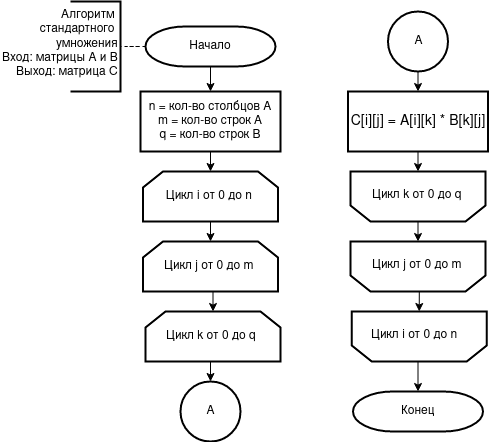
\includegraphics{def}
		\caption{Схема классического алгоритма умножения матриц}
		\label{fig:schema_bucket_1}
	\end{figure}
	
	\begin{figure}[H]
		\centering
		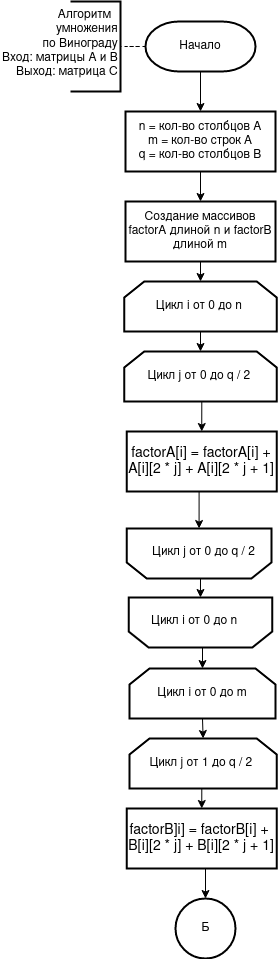
\includegraphics[width=0.38\linewidth]{vin_1}
		\caption{Схема умножения матриц алгоритмом Винограда, ч.1}
		\label{fig:schema_bucket_2}
	\end{figure}
	
	\begin{figure}[H]
		\centering
		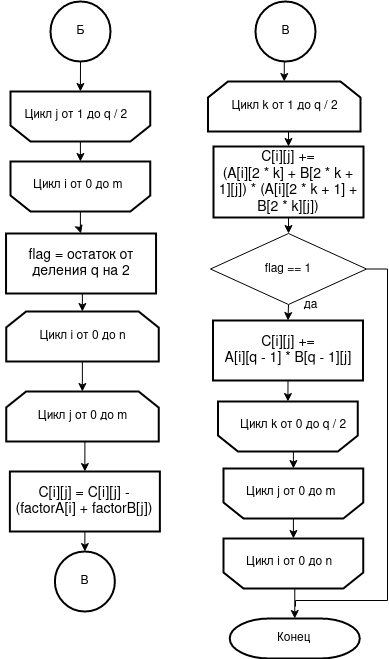
\includegraphics[width=0.75\linewidth]{vin_2}
		\caption{Схема умножения матриц алгоритмом Винограда, ч.2}
		\label{fig:schema_bucket_3}
	\end{figure}
	
	\begin{figure}[H]
		\centering
		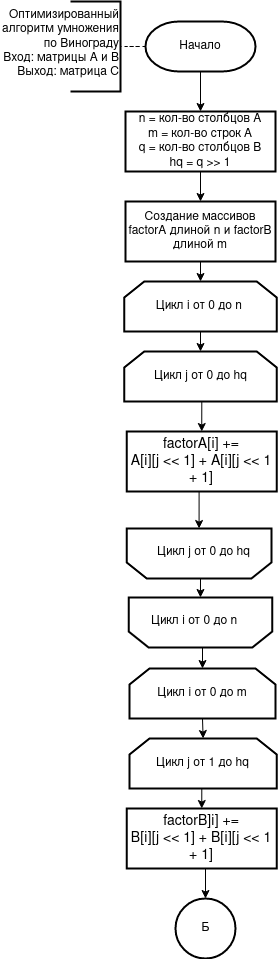
\includegraphics[width=0.38\linewidth]{opvin_1}
		\caption{Схема умножения матриц оптимизированным алгоритмом Винограда, ч.1}
		\label{fig:schema_selection}
	\end{figure}
	
	\begin{figure}[H]
		\centering
		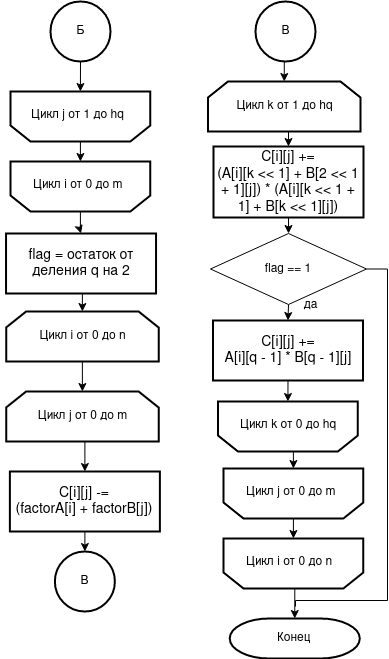
\includegraphics[width=0.75\linewidth]{opvin_2}
		\caption{Схема умножения матриц оптимизированным алгоритмом Винограда, ч.2}
		\label{fig:schema_selection}
	\end{figure}
	
	\section*{Вывод}
	
	В данном разделе были представлены описания умножения матриц классическим алгоритмом, алгоритмом Винограда и оптимизированным алгоритмом Винограда, а так же проведена оценка их трудоемкости.
	
	\chapter{Технологическая часть}
	
	В данном разделе приведены требования к ПО, обоснования выбора языка программирования, среды разработки, приведен способ замера времени выполнения, а также приведены листинги кода.
	
	\section{Требования к ПО}
	
	В программе должна присутствовать возможность:
	
	\begin{enumerate}
		\item[1)] ввода исходных матриц, участвующих в умножении;
		\item[2)] поиска матрицы, полученной в результате умножения, с помощью одного из трех рассматриваемых алгоритмов;
		\item[3)] замера процессорного времени выполнения реализаций алгоритмов.
	\end{enumerate}
	
	\section{Выбор языка программирования и среды разработки}
	
	Для реализации трех алгоритмов сортировок был выбор язык С, так как данный язык является быстродейственным.

	Средой разработки был выбран СLion. Данный выбор обусловлен тем, что данная среда предоставляет возможность разработки приложений под C/C++ и имеет инструменты для отладки кода. 
	
	\section{Выбор библиотеки и способа для замера времени}
		Для замера времени выполнения сортировок использовалась стандартная функция библиотеки <time.h> языка С~---~clock(), которая замеряет процессорное время. Если измерить время перед началом выполнения алгоритма, и после его окончания, то можно получить время выполнения функции. Реализация данной функции приведена в [1].
		
		Поскольку все процессорное время не отдается какой-либо одной задаче (в связи с явлением вытеснения процессов из ядра, квантование процессорного времени), то требуется усреднить результаты вычислений: замерить совокупное время выполнения реализации алгоритма N раз и вычислить среднее время выполнения.
		
	\section{Реализации алгоритмов}
	
	В листингах \ref{lev},\ref{damlev},\ref{damlevrec} приведены реализации алгоритмов умножения матриц классическим методом, Винограда и оптимизорованного Винограда соответсвенно.
	
	\begin{lstlisting}[label=lev,caption=Листинг алгоритма классического умножения матриц,language=C]
		matrix_t *mul_matrix_def(matrix_t *first_mat, matrix_t *second_mat)
		{
		    matrix_t *res = create_matrix(first_mat->rows, second_mat->cols);

		    int eq_dim = first_mat->cols;

		    for (int i = 0; i < res->rows; ++i) {
			for (int j = 0; j < res->cols; ++j) {
			    (res->elements)[i][j] = 0;
			    for (int k = 0; k < eq_dim; ++k) {
				(res->elements)[i][j] += (first_mat->elements)[i][k] * (second_mat->elements)[k][j];
			    }
			}
		    }

		    return res;
		}
	\end{lstlisting}

	
	\begin{lstlisting}[label=damlev,caption=Листинг алгоритма Винограда умножения матриц,language=C]
		matrix_t *mul_matrix_vinograd(matrix_t *first_mat, matrix_t *second_mat)
		{
		    matrix_t *res = create_matrix(first_mat->rows, second_mat->cols);
		    int *factorA = calloc(first_mat->rows, sizeof(int));
		    int *factorB = calloc(second_mat->cols, sizeof(int));

		    int eq_dim = first_mat->cols;

		    for (int i = 0; i < first_mat->rows; ++i)
			for (int j = 0; j < eq_dim / 2; ++j)
			    factorA[i] = factorA[i] + (first_mat->elements)[i][2 * j] * (first_mat->elements)[i][2 * j + 1];

		    for (int i = 0; i < second_mat->cols; ++i)
			for (int j = 0; j < eq_dim / 2; ++j)
			    factorB[i] = factorB[i] + (second_mat->elements)[2 * j][i] * (second_mat->elements)[2 * j + 1][i];

		    for (int i = 0; i < res->rows; ++i) {
			for (int j = 0; j < res->cols; ++j) {
			    (res->elements)[i][j] = -factorA[i] - factorB[j];
			    for (int k = 0; k < eq_dim / 2; ++k) {
				(res->elements)[i][j] = (res->elements)[i][j] + ((first_mat->elements)[i][2 * k] + (second_mat->elements)[2 * k + 1][j]) * ((first_mat->elements)[i][2 * k + 1] + (second_mat->elements)[2 * k][j]);
			    }
			}
		    }

		    if (eq_dim % 2 != 0) {
			for (int i = 0; i < res->rows; ++i)
			    for (int j = 0; j < res->cols; ++j)
				(res->elements)[i][j] = (res->elements)[i][j] + (first_mat->elements)[i][first_mat->cols - 1] * (second_mat->elements)[second_mat->rows - 1][j];
		    }

		    free(factorA);
		    free(factorB);

		    return res;
		}
	\end{lstlisting}
	
	\bigbreak

	\begin{lstlisting}[label=damlevrec,caption=Листинг оптимизированного алгоритма Винограда умножения матриц,language=C]
		matrix_t *mul_matrix_vinograd_optimized(matrix_t *first_mat, matrix_t *second_mat)
		{
		    matrix_t *res = create_matrix(first_mat->rows, second_mat->cols);
		    int *factorA = calloc(first_mat->rows, sizeof(int));
		    int *factorB = calloc(second_mat->cols, sizeof(int));

		    int eq_dim = first_mat->cols;
		    int half_eq_dim = eq_dim >> 1;

		    for (int i = 0; i < first_mat->rows; ++i)
			for (int j = 0; j < half_eq_dim; ++j)
			    factorA[i] += (first_mat->elements)[i][j << 1] * (first_mat->elements)[i][(j << 1) + 1];

		    for (int i = 0; i < second_mat->cols; ++i)
			for (int j = 0; j < half_eq_dim; ++j)
			    factorB[i] += (second_mat->elements)[j << 1][i] * (second_mat->elements)[(j << 1) + 1][i];

		    for (int i = 0; i < res->rows; ++i) {
			for (int j = 0; j < res->cols; ++j) {
			    (res->elements)[i][j] = -factorA[i] - factorB[j];
			    for (int k = 0; k < half_eq_dim; ++k) {
				(res->elements)[i][j] += ((first_mat->elements)[i][k << 1] + (second_mat->elements)[(k << 1) + 1][j]) * ((first_mat->elements)[i][(k << 1) + 1] + (second_mat->elements)[(k << 1)][j]);
			    }
			}
		    }

		    if (eq_dim % 2 != 0) {
			for (int i = 0; i < res->rows; ++i)
			    for (int j = 0; j < res->cols; ++j)
				(res->elements)[i][j] += (first_mat->elements)[i][first_mat->cols - 1] * (second_mat->elements)[second_mat->rows - 1][j];
		    }

		    free(factorA);
		    free(factorB);

		    return res;
		}
	\end{lstlisting}

	\section{Тестирование алгоритмов}

	В таблице~\ref{tbl:test} приведены тесты для функций, реализующих алгоритмы классического умножения матриц, умножения алгоритмом Винограда и оптимизированного Винограда. Все тесты пройдены успешно.
	
	\begin{table}[h!]
		\begin{center}
			\caption{\label{tbl:test} Тестирование трех рассматриваемых алгоритмов умножения матриц для разных входный данных}
			\begin{tabular}{|c|c|c|}
				\hline
				Первая матрица & Вторая матрица & Ожидаемый результат \\ 
				\hline
			$\begin{pmatrix}
			1 & 2 & 3\\
			1 & 2 & 3\\
			1 & 2 & 3
			\end{pmatrix}$ &
			$\begin{pmatrix}
			1 & 2 & 3\\
			1 & 2 & 3\\
			1 & 2 & 3
			\end{pmatrix}$ &
			$\begin{pmatrix}
			6 & 12 & 18\\
			6 & 12 & 18\\
			6 & 12 & 18
			\end{pmatrix}$ \\\hline
			$\begin{pmatrix}
			1 & 2 & 3\\
			1 & 2 & 3
			\end{pmatrix}$ &
			$\begin{pmatrix}
			1 & 2\\
			3 & 4\\
			5 & 6
			\end{pmatrix}$ &
			$\begin{pmatrix}
			22 & 28\\
			22 & 28
			\end{pmatrix}$ \\\hline
			$\begin{pmatrix}
			2
			\end{pmatrix}$ &
			$\begin{pmatrix}
			3
			\end{pmatrix}$ &
			$\begin{pmatrix}
			6
			\end{pmatrix}$ \\\hline
			$\begin{pmatrix}
			1 & 2 & 3\\
			1 & 2 & 3\\
			1 & 2 & 3
			\end{pmatrix}$ &
			$\begin{pmatrix}
			-1 & -2 & -3\\
			1 & 2 & 3\\
			1 & 2 & 3
			\end{pmatrix}$ &
			$\begin{pmatrix}
			4 & 8 & 12\\
			4 & 8 & 12\\
			4 & 8 & 12
			\end{pmatrix}$\\\hline
			\end{tabular}			
		\end{center}
	\end{table}

	\section*{Вывод}
	
	В данном разделе были разработаны исходные коды алгоритмов классического умножения матриц, умножения алгоритмом Винограда и оптимизированного Винограда.
	
	\chapter{Экспериментальная часть}
	
	\section{Технические характеристики}
	
	Ниже приведены технические характеристики устройства, на котором было проведено тестирование ПО:
	
	\begin{enumerate}
		\item[1)] операционная система Windows-10, 64-bit;
		\item[2)] оперативная память 16 ГБ;
		\item[3)] процессор Intel(R) Core(TM) i7-8565U CPU @ 1.80 ГГц, 4 ядра, 8 логических процессоров.
	\end{enumerate}
	
	\section{Замеры времени}
	
	Введем обозначения: Def -- классический алгоритм умножения матриц, Vin -- умножение матриц алгоритмом Винограда, OpVin -- умножение матриц оптимизированным алгоритмом Винограда.
	Все рассматриваемые в этом разделе матрицы -- квадратные.
	
	В таблице \ref{table:t1} приведены результаты замеров времени алгоритмов для входных матриц, имеющих различные четные размеры.
	
	\begin{table} [H]
		\caption{Таблица замера времени выполнения алгоритмов на входных матрицах, имеющих четные размеры}
		\label{table:t1}
		\begin{center}
			\begin{tabular}{|c | c | c | c |}
				
				\hline
				
				Количество строк и столбцов & Def & Vin & OpVin \\ [0.5ex]
				
				\hline
				
				50 & 835 & 623 & 536 \\ 
				
				\hline 
				
				100 & 5678 & 4446 & 4155\\ 
				
				\hline 
				
				200 & 45255 & 41572 & 34487\\ 
				
				\hline 
				
				300 & 155263 & 129265 & 126086\\ 
				
				\hline 
			\end{tabular}
		\end{center}
	\end{table}

	Зависимость времени работы алгоритмов умножения матриц от четных размеров умножаемых матриц представлена на рис. \ref{ris1}.

	\begin{center}
		\begin{figure}[H]
		\center
		\begin{tikzpicture}
				\begin{axis} [
					legend pos = north west,
					grid = major,
					xmin = 0,
					ymin = 0, 
					xmax = 300,
					ymax = 156000,
					xlabel = $\text{размеры (количество строк и столбцов)}$,
					ylabel = $\text{время (мс)}$
					]
					\legend{ 
						$Def$, 
						$Vin$,
						$OpVin$
					};
					\addplot coordinates {
						(50,835) (100,5678) (200,45255) (300,155263) };
					\addplot coordinates {
						(50,623) (100,4446) (200,41572) (300,129265) };
					\addplot coordinates {
						(50,536) (100,4155) (200,34487) (300,126086) };
				\end{axis}
		\end{tikzpicture}
		\caption{Зависимость времени от размера входных матриц}
		\label{ris1}
		\end{figure}
	\end{center}
	
	
	В таблице \ref{table:t2} приведены результаты замеров времени алгоритмов для входных матриц, имеющих различные нечетные размеры.
	
	\begin{table} [H]
		\caption{Таблица замера времени выполнения алгоритмов на входных матрицах, имеющих нечетные размеры}
		\label{table:t2}
		\begin{center}
			\begin{tabular}{|c | c | c | c |}
				
				\hline
				
				Количество строк и столбцов & Def & Vin & OpVin \\ [0.5ex]
				
				\hline
				
				51 & 695 & 614 & 574 \\ 
				
				\hline 
				
				101 & 5928 & 4484 & 4324\\ 
				
				\hline 
				
				201 & 44531 & 36619 & 34975\\ 
				
				\hline 
				
				301 & 158599 & 135065 & 133109\\ 
				
				\hline 
			\end{tabular}
		\end{center}
	\end{table}

	Зависимость времени работы алгоритмов умножения матриц от нечетных размеров умножаемых матриц представлена на рис. \ref{ris2}.

	\begin{center}
		\begin{figure}[H]
		\center
		\begin{tikzpicture}
				\begin{axis} [
					legend pos = north west,
					grid = major,
					xmin = 0,
					ymin = 0, 
					xmax = 301,
					ymax = 159000,
					xlabel = $\text{размеры (количество строк и столбцов)}$,
					ylabel = $\text{время (мс)}$
					]
					\legend{ 
						$Def$, 
						$Vin$,
						$OpVin$
					};
					\addplot coordinates {
						(51,695) (101,5928) (201,44531) (301,158599) };
					\addplot coordinates {
						(51,614) (101,4484) (201,36619) (301,135065) };
					\addplot coordinates {
						(51,574) (101,4324) (201,34975) (301,133109) };
				\end{axis}
		\end{tikzpicture}
		\caption{Зависимость времени от размера входных матриц}
		\label{ris2}
		\end{figure}
	\end{center}
	

	\section*{Вывод}
	
	Результаты замеров показали, что алгоритм Винограда и оптимизированный алгоритм Винограда работают быстрее классического алгоритма умножения матриц за счет того, что в них меньше операций умножения. При этом оптимизированный алгоритм Винограда работает немного быстрее обычного алгоритма Винограда за счет введеных оптимизаций. 
	
	\chapter*{Заключение}
	
	Цель лабораторной работы достигнута -- были изучены и реализованы алгоритмы умножения матриц классическим методом, Виноградом и оптимизированным Виноградом. Все задачи решены:
	
	\begin{enumerate}
		\item[1)] были изучены и рассмотрены алгоритмы классического умножения матриц, алгоритм Винограда и модифицированный алгоритм Винограда;
		\item[2)] были построены блок-схемы данных алгоритмов;
		\item[3)] был реализован каждый из алгоритмов;
		\item[4)] была оценена их трудоемкость;
		\item[5)] были экспериментально получены временные характеристики алгоритмов;
		\item[6)] были сделаны выводы на основании проделанной работы
	\end{enumerate}
	
	На основании проведенных экспериментов и оценки трудоемкости было определено, что оптимизированный алгоритм Винограда умножения матриц имеет меньшую сложность, нежели классический алгоритм. При этом алгоритм Винограда обгоняет простой алгоритм в среднем в 1.3 раза, а оптимизированный алгоритм Винограда -- в 1.6 раз. При этом для обоих алгоритмов Винограда требуется выделение дополнительной памяти. 
	
\addcontentsline{toc}{chapter}{Список использованных источников}

\nocite{*} 

\renewcommand\bibname{Список использованных источников} % переименовать страницу списка литературы
\bibliographystyle{utf8gost705u}  % стилевой файл для оформления по ГОСТу
\bibliography{lib}          % имя библиографической базы (bib-файла)
	
\end{document}
